\documentclass{jsarticle}

\usepackage{listings,jlisting}
\usepackage[dvipdfmx]{graphicx}
\usepackage{bmpsize}

\lstset{
    basicstyle={\ttfamily},
    identifierstyle={\small},
    commentstyle={\smallitshape},
    keywordstyle={\small\bfseries},
    ndkeywordstyle={\small},
    stringstyle={\small\ttfamily},
    frame={tb},
    breaklines=true,
    columns=[l]{fullflexible},
    numbers=left,
    xrightmargin=0zw,
    xleftmargin=3zw,
    numberstyle={\scriptsize},
    stepnumber=1,
    numbersep=1zw,
    lineskip=-0.5ex
}
\begin{document}

\title{計算機科学実験及演習4 エージェント 課題1}
\author{1029-28-2473 二見 颯}
\maketitle

\section{プログラム概要}
データ点が書かれたファイルを読み込み、SVM の識別器を作成してそのパラメータを出力する。
作成した SVM によりクラスの予測を行い、与えられたデータ点と予測された識別境界を平面上にプロットする。

\section{外部仕様}
\begin{itemize}
    \item main.py - プログラムのエントリポイント。svc.py の SVClassifier および utils.py の関数を参照している
    \item svc.py - SVM のクラス SVClassifier を実装
    \item utils.py - ファイル読み込み(load\_data)と結果のプロット(plot\_decision\_regions)を実装
\end{itemize}
プログラムの実行は \\
{\bf ./main.py [入力ファイルへのパス] [カーネルトリックの種類] [カーネルトリックのパラメータ]}\\
カーネルトリックの種類については、n でカーネルトリックなし、p で多項式カーネル、g でガウスカーネル、
s でシグモイドカーネルとする。
プログラム引数が正しくない形式の場合は、エラーとしてプログラムが終了する。
\begin{lstlisting}
$ ./main.py data/square.dat n
    pcost       dcost       gap    pres   dres
0: -1.2457e-01 -3.5986e-01  2e-01  7e-18  1e+00
1: -1.2497e-01 -1.2743e-01  2e-03  5e-17  3e-02
2: -1.2500e-01 -1.2502e-01  2e-05  2e-17  3e-04
3: -1.2500e-01 -1.2500e-01  2e-07  4e-17  3e-06
4: -1.2500e-01 -1.2500e-01  2e-09  3e-17  3e-08
Optimal solution found.
alpha: 
0 [0.0625]
1 [0.0625]
2 [0.0625]
3 [0.0625]
theta candidates:  [0.9999999680249498, 1.0, 0.9999999680249498, 1.0]
SVClassifier W = [0.49999999 0.        ], θ = 0.9999999840124749
[グラフ出力]
\end{lstlisting}
必要なライブラリ等は以下
\begin{lstlisting}
Python 3.6.1 :: Anaconda custom (64-bit)
numpy 1.14.2
cvxopt 1.2.1
tqdm 4.26.0
matplotlib 2.0.2
\end{lstlisting}

\section{内部仕様}
\underline{svc.py}
\subsection*{SVClassifierクラス}
サポートベクタマシンを定義する.
privateメンバ
\begin{itemize}
    \item X, y - 訓練データ点とその正解クラス
    \item n - 訓練データの個数
    \item kf - kernel trickとして用いる関数(kernel function)
    \item p, q - kernel functionのパラメータ(optional)
    \item alpha, theta - SVMの内部パラメータであり、それぞれsetLagrange関数, setClassifier関数で
    決定する
\end{itemize}
コンストラクタにより、kf, p, qを決定する
\subsection*{fit}
X, y, nを決定して、alpha, thetaを決定する各関数を呼び出す \\
@param[in] X, y

\subsection*{\_setLagrange}
以下の2次計画問題をcvxopt.solvers.qpを用いて解くことで、alphaを決定する \\

\subsection*{\_setClassifier}
alphaとx, yからthetaを決定して、"W = , $\theta$ = "の形で識別器を出力する \\

\subsection*{\_kernelPolynomial}
多項式カーネル

\subsection*{\_kernelGauss}

\subsection*{\_kernelSigmoid}

\subsection*{predict}
SVMによりtXのクラスの予測をする \\
@param[in] tX テストデータ


\underline{utils.py}
\subsection*{load\_data}
filepathにあるsample\_linear.dat同様の形式のデータをX,yに読み込む \\
@param[in] filepath \\
@return X, y \\
入力ファイルのデータ点は、行の最後に正解クラスが指定される以下のような形式で与えられる。
\begin{lstlisting}
1.0, 0.5, 1
0.5, 0.25, -1
\end{lstlisting}
1行ごとに", "でsplitして処理するためデータ点がn次元の特徴で表せる場合にも対応できる。

\subsection*{plot\_decision\_regions}
xを2次元平面にplotする.
plotされた点の色はyによって決まり、領域の色はmodelの予測結果により決まる \\
@param[in] x, y, model, resolution resolutionによりグリッドの幅を指定する \\
@return なし \\
xが2次元でない場合、この関数は終了する。\\
x=(x1, x2)に対する正解クラスをy, SVMによる予測クラスをzとする。x1の最小値-1から最大値+1, x2の最小値-1から最大値+1の範囲で
グリッド点を作成して、そのグリッド点に対してmodel.predictすることでzの決定領域が得られる。\\
その後、各xの点をyに応じた色(red, blue)と形(o, x)でplotする。

\section{評価結果}
% sklearn で確認したい
\subsection{sample\_linear.dat}
\begin{figure}[!h]
\centering 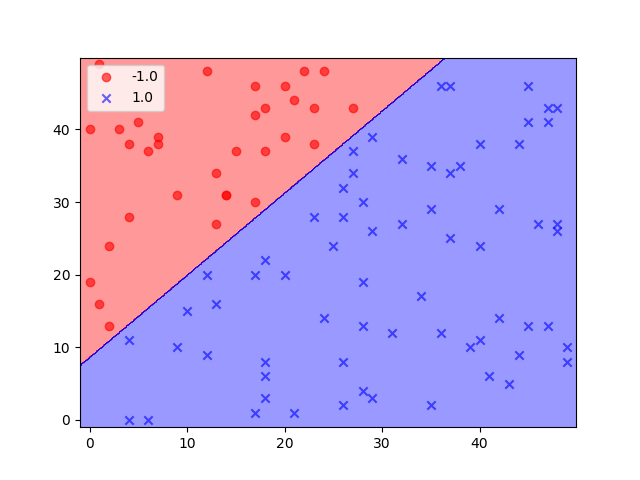
\includegraphics[width=15cm]{sample_linear.png}
\caption{sample\_linear.dat}
\end{figure}

\subsection{sample\_circle.dat}
\subsection{poly\_five.dat}
1次元データx=[1, 2, 5, 7, 8], y=[1, 1, -1, -1, 1]をpoly\_five.datとする。
このとき、$\alpha$について以下のような結果が得られた。
\begin{lstlisting}
alpha: 
0 [2.86101852e-09]
1 [1.01333335]
2 [8.47919771e-08]
3 [4.07999985]
4 [3.06666658]
\end{lstlisting}

\section{考察}
SVClassifier.predict の実装について、はじめは
\begin{lstlisting}
def predict(self, tX):
    batch_size = tX.shape[0]
    preds = []
    for i in range(batch_size):
        res = 0
        for j in range(self.__n):
            res += self.__alpha[j] * self.__y[j] * self.__kf(self.__X[j], tX[i])
        res -= self.__theta
        preds.append(np.sign(res))
    return np.array(preds)
\end{lstlisting}
のように実装していたが、この場合for文を2重に

\section{参考資料}
\begin{itemize}
    \item Python機械学習プログラミング Sebastian Raschka 著
    \item はじめてのパターン認識 平井 有三 著
\end{itemize}

\end{document}